\subsection{Calibration Frame Preparation}

For each camera location of the dataset, a set of calibration frames (generally fifteen,
location dependant) and corresponding binary masks were prepared.
The frames were extracted from location-specific reference videos supplied with the dataset
consisting of a person standing, facing the camera, at known distance intervals
and holding a sheet of A4 paper labelled with the corresponding distance.

\subsubsection{Frame Extraction}
In an effort to streamline the frame extraction process, an extractor program was created
(Figure~\ref{fig:frame_extractor}).
This tool enabled reference videos to be dragged and dropped into a GUI window allowing for the
easy navigation between individual frames to extract the optimal one for each distance.
With this software, the next/previous frames are accessed with the 'left'/'right' arrow keys, the frame
index position is moved ahead/behind 20 places with the 'd'/'a' keys and the frame found at a specific
timestamp is accessed with the 's' key followed by entering a time (in seconds) into an input bar.
The active frame (at the current index) can be saved to disk with the 'enter' key followed by entering
a filename in an input bar.
\vspace{5mm}

\begin{figure}[htbp]
    \centering
    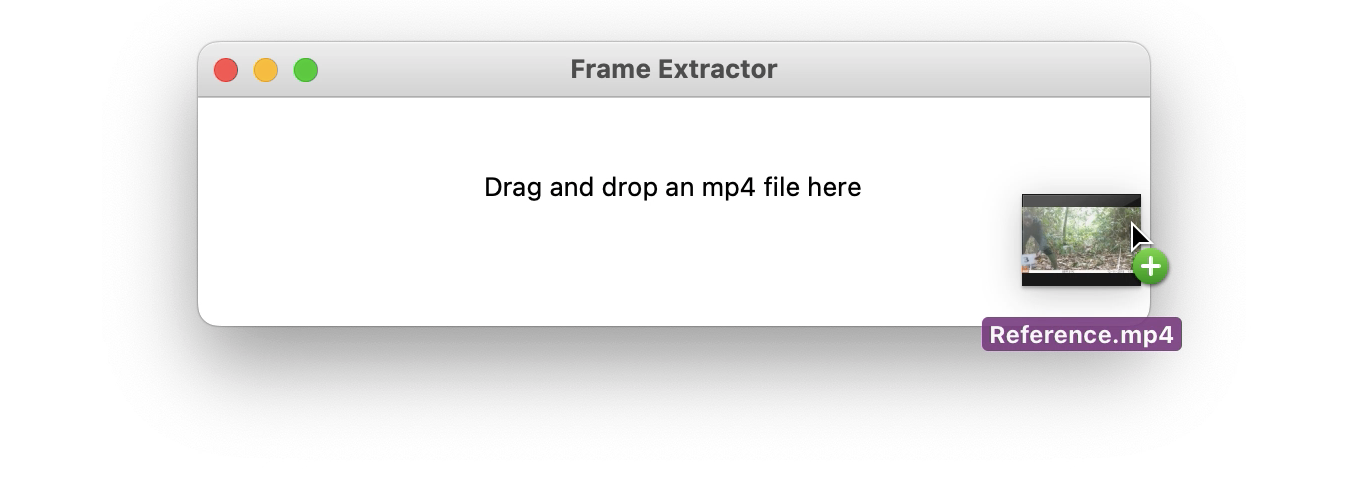
\includegraphics[scale=0.5]{body/experimental/assets/frame_extractor/drag_drop}
    \vspace{-3mm}
    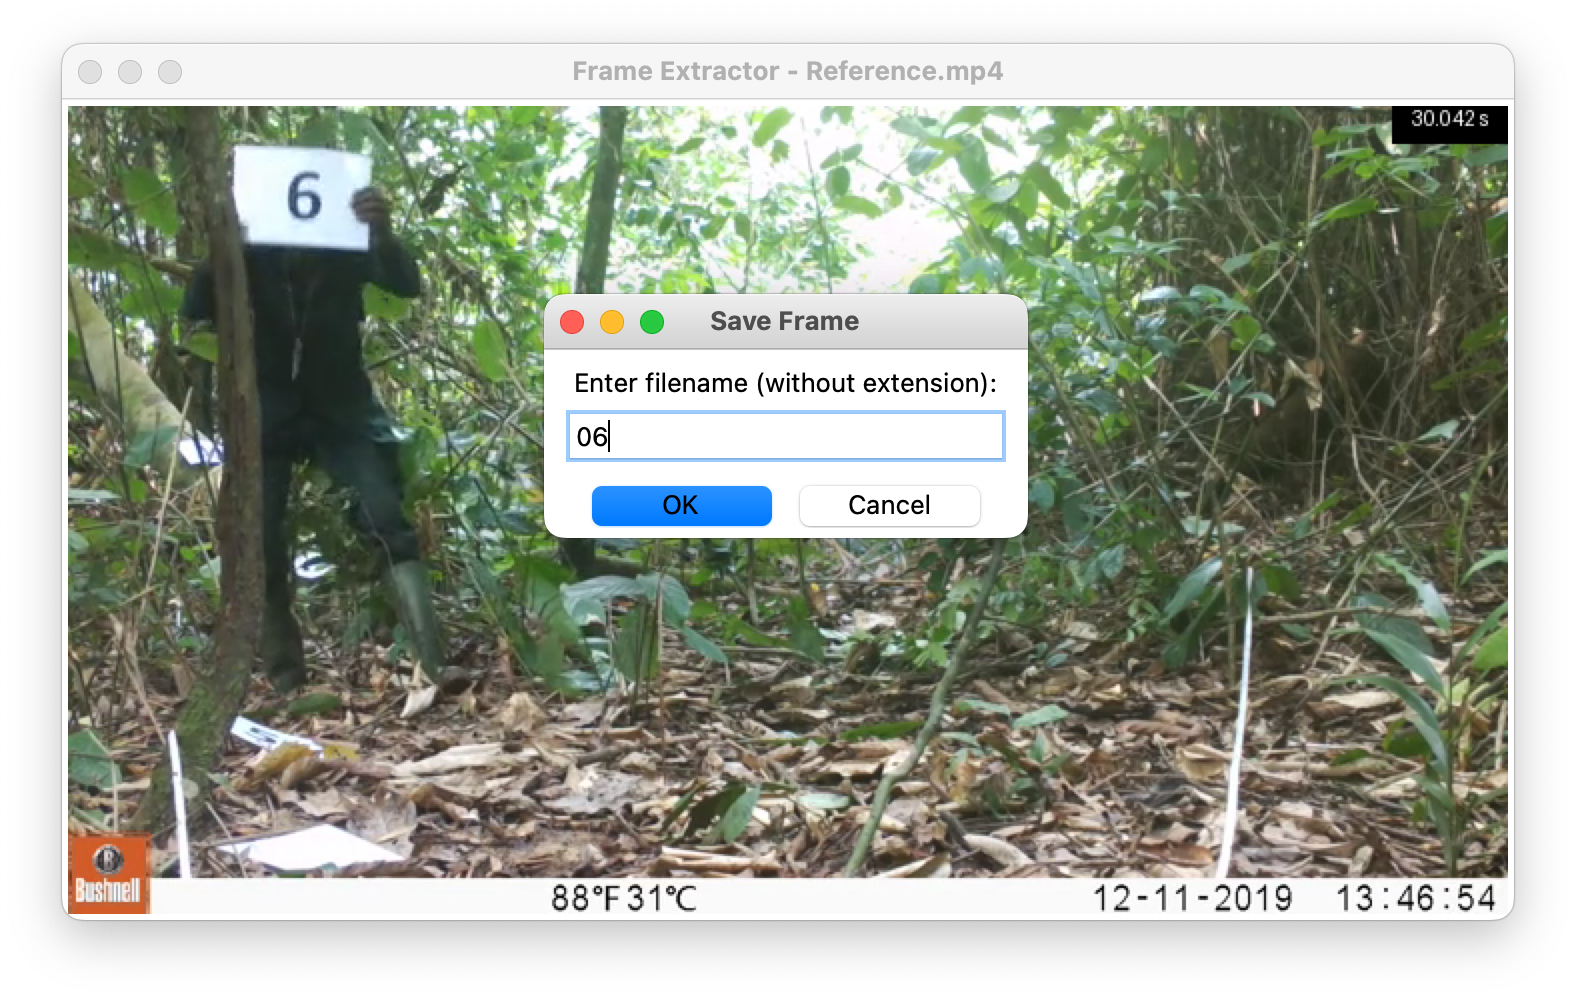
\includegraphics[scale=0.5]{body/experimental/assets/frame_extractor/save_frame}
    \caption{Frame extractor program showing the drag/drop (top) and save frame (bottom) features}
    \label{fig:frame_extractor}
\end{figure}

\clearpage

\subsubsection{Frame Mask Creation}\label{subsubsec:mask_creation}

For each of the extracted calibration frames, a corresponding binary mask was created.
This task can be completed manually using image manipulation software (e.g.\ Photoshop,
GIMP, etc\ldots) where the segmentation boundary is manually traced then filled.
This approach, however, is rather labour-intensive, constituting somewhat
of a bottleneck, and therefore it is desirable to automate the process.

To assess the feasibility of automation, a two-stage detection/segmentation pipeline was
created.
Here, raw calibration frames are first processed with YOLOv5 detector\cite{YOLO} to
generate bounding boxes (prompted to detect humans) enclosing the frame landmarks.
The bounding boxes are then passed to Segment Anything Model which predicts segmentation
masks for the landmarks.

The efficacy of this automated method of calibration frame mask generation was tested on
several raw calibration frames.
Two examples of the raw calibration frames (Figure~\ref{fig:raw_frames}) along with their
corresponding manual (Figure~\ref{fig:manual_masks}) and automated (Figure~\ref{fig:sam_masks})
masks are shown below.

\begin{figure}[htbp]
    \centering
    \makebox[0.8\textwidth][c]{
        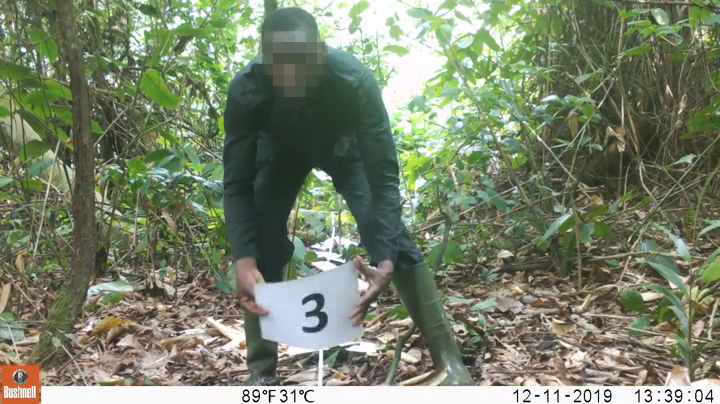
\includegraphics[width=0.9\textwidth]{body/experimental/assets/frame_masks/close_blurred}
    }\\[1mm]
    \makebox[0.8\textwidth][c]{
        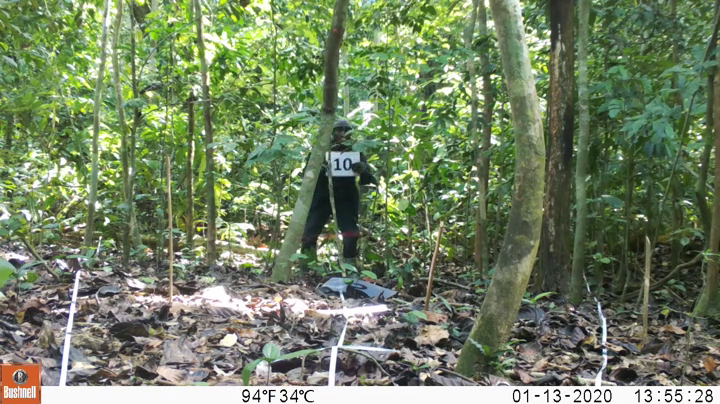
\includegraphics[width=0.9\textwidth]{body/experimental/assets/frame_masks/far}
    }
    \caption{Raw calibration frames}
    \label{fig:raw_frames}
\end{figure}

\begin{figure}[htbp]
    \centering
    \makebox[0.8\textwidth][c]{
        
\includegraphics[width=0.9\textwidth]{body/experimental/assets/frame_masks/close_manual_mask}
    }\\[1mm]
    \makebox[0.8\textwidth][c]{
        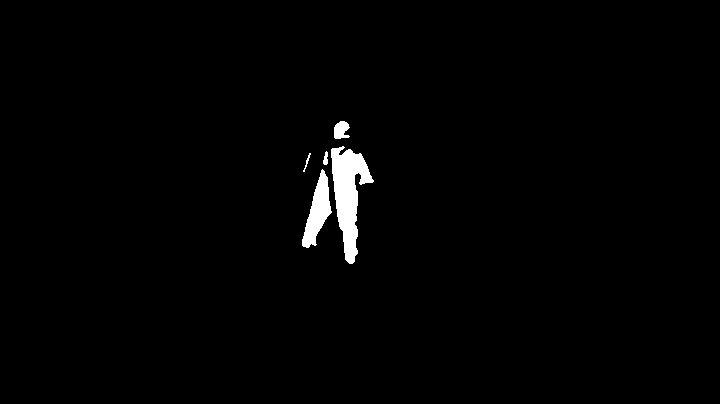
\includegraphics[width=0.9\textwidth]{body/experimental/assets/frame_masks/far_manual_mask}
    }
    \caption{Manual calibration frame masks}
    \label{fig:manual_masks}
\end{figure}

\begin{figure}[htbp]
    \centering
    \makebox[0.8\textwidth][c]{
        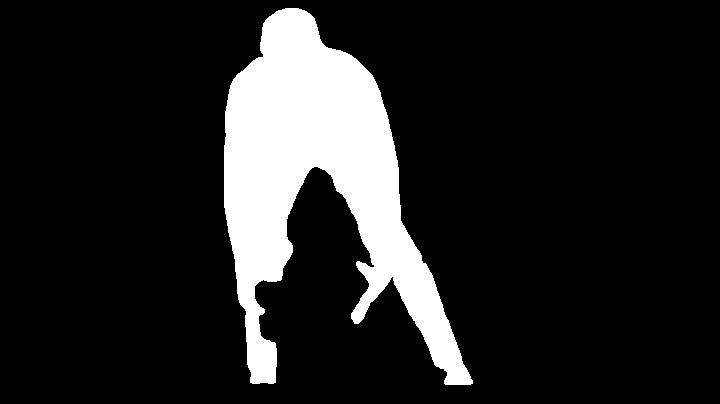
\includegraphics[width=0.9\textwidth]{body/experimental/assets/frame_masks/close_sam_mask}
    }\\[1mm]
    \makebox[0.8\textwidth][c]{
        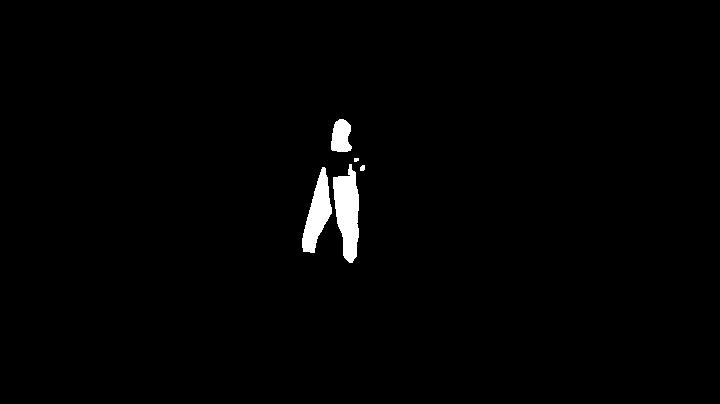
\includegraphics[width=0.9\textwidth]{body/experimental/assets/frame_masks/far_sam_mask}
    }
    \caption{Automated calibration frame masks}
    \label{fig:sam_masks}
\end{figure}




